\section{Introduction}
\label{sec:intro}

Modern energy processes---supercritical power plants, combined-cycle units, and district heating systems---must satisfy hard constraints on pressure, temperature, enthalpy, and power output across wide operating ranges. Coal quality variation, heat exchanger fouling, equipment degradation, and load-following requirements introduce significant discrepancies between the nominal design model and the true plant dynamics~\cite{astrom2000boiler,tan2006supercritical}. Under such model mismatch, a controller optimized for nominal conditions may violate physical constraints, potentially causing equipment damage, forced outages, or safety incidents.

Model predictive control (MPC) is the dominant constrained control approach in the process industries, with over 90\% of industrial applications in process control including power generation~\cite{qin2003survey,mayne2000constrained}. MPC handles constraints explicitly within a receding-horizon optimization and can incorporate disturbance estimation for offset-free tracking~\cite{morari1999model}. However, MPC provides safety guarantees only within its finite prediction horizon; it does not offer formal forward invariance guarantees that extend beyond the horizon. Robust and stochastic MPC variants~\cite{hewing2020cautious} add probabilistic constraint tightening but at substantially higher computational cost, and their guarantees depend on the accuracy of the uncertainty description over the full horizon.

Control barrier functions (CBFs)~\cite{ames2017cbf} provide an alternative safety mechanism: a CBF defines a safe set and enforces forward invariance through a quadratic program (QP) that projects potentially unsafe actions to the nearest safe action at each time step. The CBF-QP framework guarantees safety under the assumption that the dynamics model used to compute the constraint is exact. For process constraints with high relative degree (e.g., steam pressure, which requires two Lie derivatives to reach the control input), high-order CBFs (HOCBFs)~\cite{xiao2021hocbf} extend the CBF construction through a recursive $\psi$-chain. However, under model mismatch---the norm in industrial practice---the nominal HOCBF constraint becomes incorrect, and the QP may certify unsafe actions as safe~\cite{taylor2020issf}.

Gaussian processes (GPs) offer a principled framework for learning model residuals from data with calibrated uncertainty quantification~\cite{rasmussen2006gp}. Several works combine GPs with CBFs for robust safety~\cite{cheng2019guaranteed,fisac2018general}, but existing GP-CBF methods apply the GP uncertainty only at the top-level CBF constraint ($m=1$) or aggregate it over an MPC prediction horizon. For process constraints with relative degree $m \geq 2$, the model residual propagates through successive Lie derivatives and a single top-level uncertainty bound is structurally incomplete---it cannot capture the amplification of uncertainty through the HOCBF $\psi$-chain.

\textbf{Contributions.} This paper introduces a Robust HOCBF safety filter for energy process control under model mismatch. The three contributions are:

\begin{enumerate}
    \item \textbf{Robust HOCBF with compositional uncertainty propagation.} A GP-augmented safety filter in which GP mean correction reduces the residual perturbation, and a recursive $\sigma$-chain propagates per-dimension GP posterior uncertainties through all $m$ levels of the HOCBF $\psi$-chain, yielding a per-constraint, relative-degree-aware robustness margin $\epsilon(x)$. Under Assumption $\Delta g = 0$ (exact input matrix) and a fixed GP with $\kappa_\epsilon = 1$, Theorem~1 establishes forward invariance with probability $\geq 1-\delta$.

    \item \textbf{Process-control-oriented safety certification and sampled-data implementation.} We provide explicit conditions for QP feasibility (Proposition~1), analyze the sampled-data implementation gap between the continuous-time certificate and discrete-time execution, and characterize the one-sided diagnostic limitation of QP infeasibility as a calibration indicator. The filter is policy-agnostic: any Lipschitz-continuous upstream controller receives the same safety guarantee.

    \item \textbf{Validation on a 5th-order supercritical boiler-turbine benchmark.} Under $\Phi$-scaled nonlinear dynamics with six static perturbation scenarios and nominal operation, the Robust HOCBF transforms nominal HOCBF failure ($>95\%$ violation) to no observed CBF violations. Under additional unseen time-varying disturbances, it achieves substantially lower violation than the implemented NMPC baseline. The filter is validated with both a classical LQR controller and a PPO-trained policy, confirming that safety is delivered by the filter rather than the policy class.
\end{enumerate}

Online GP adaptation and differentiable QP-based policy distillation are discussed as implementation enhancements (Sections~\ref{sec:deployment} and~\ref{sec:results}) but are not co-equal scientific contributions.

\begin{figure*}[t]
    \centering
    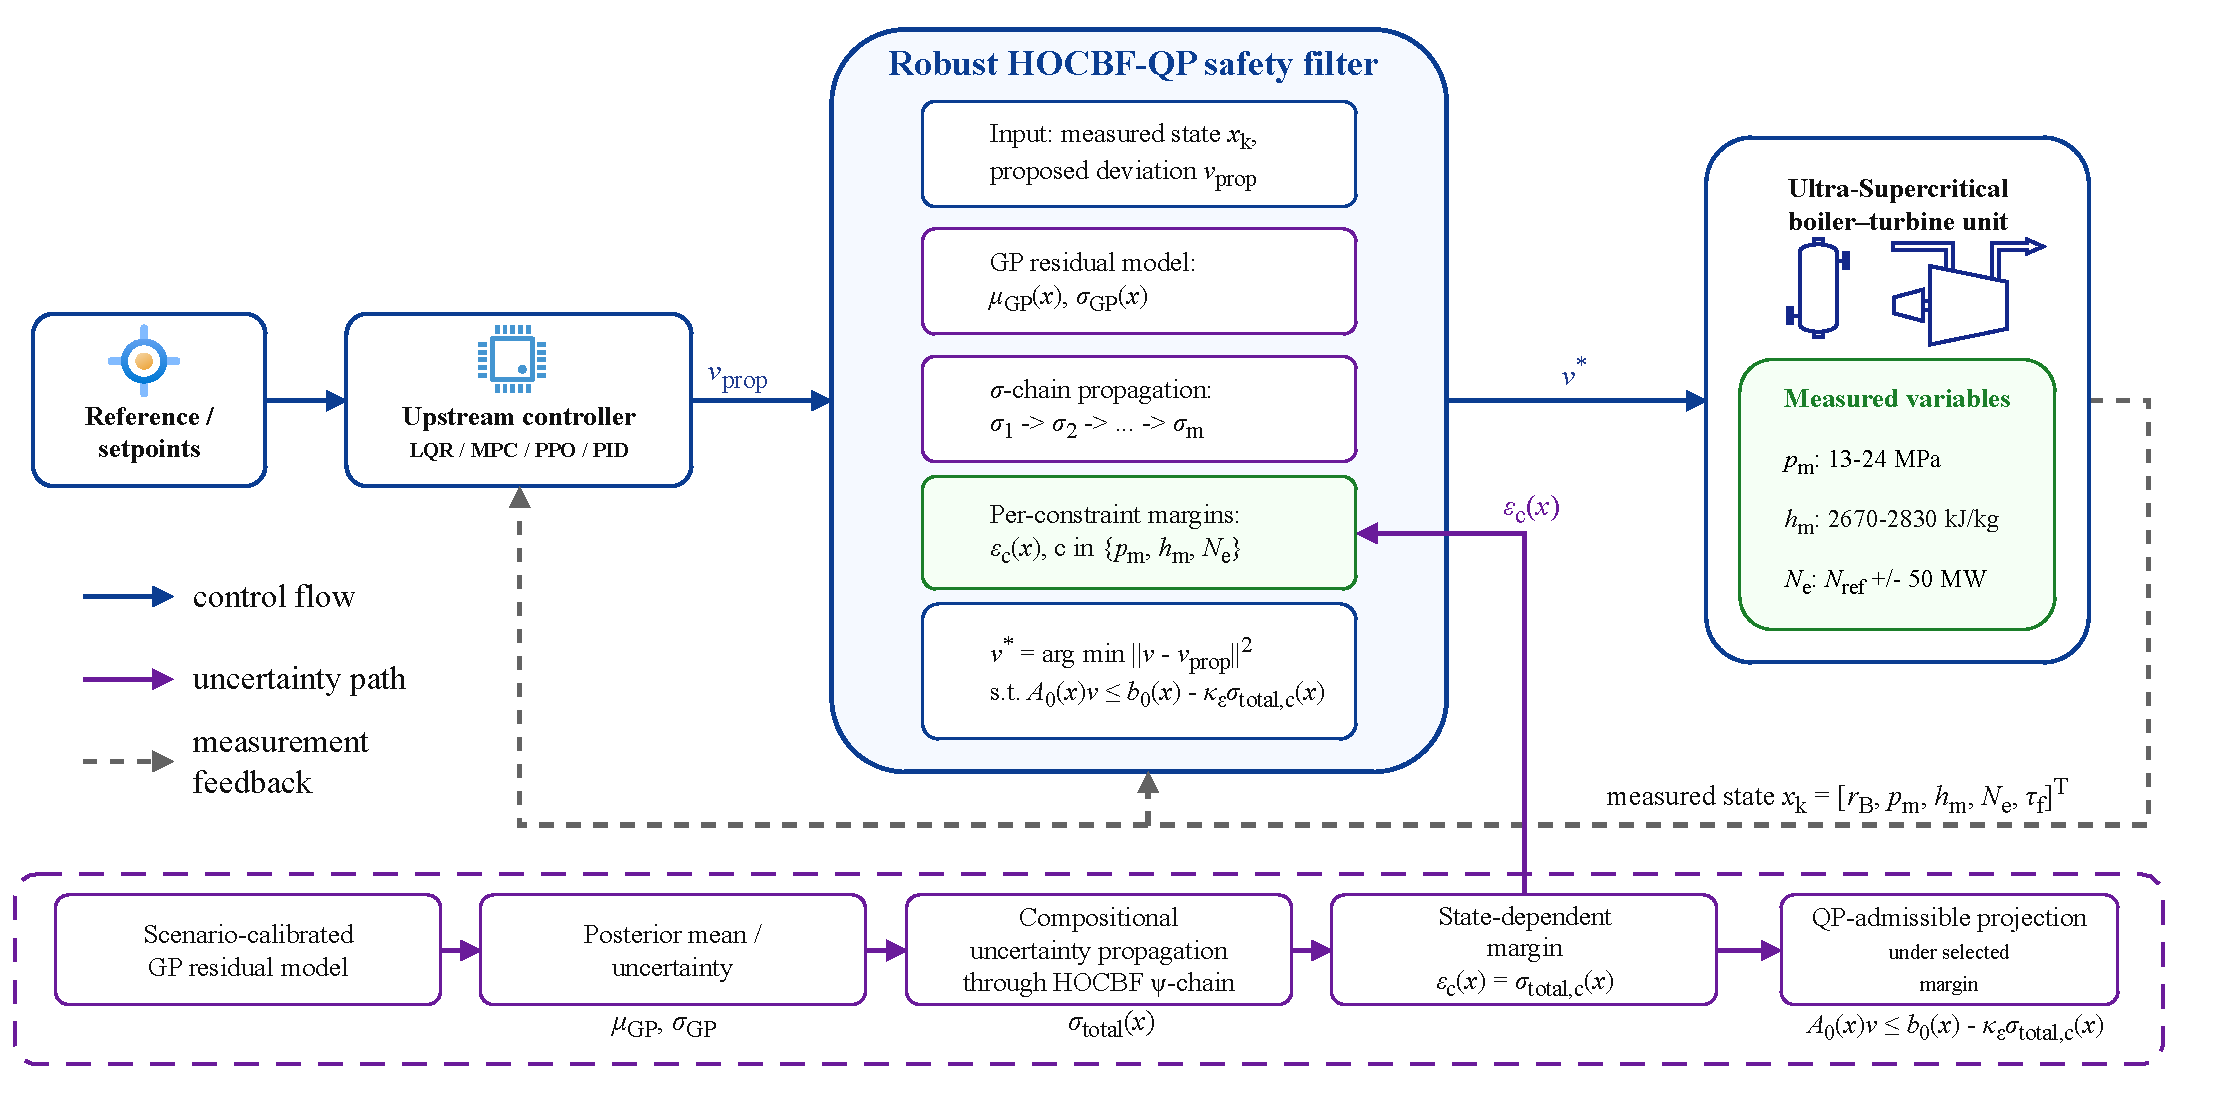
\includegraphics[width=0.92\textwidth]{figures/Figure_1.pdf}
    \caption{Process-control-oriented architecture of the Robust HOCBF safety filter. An upstream controller (LQR, MPC, PPO, or classical) proposes an action $u_{\mathrm{prop}}$; the Robust HOCBF-QP projects it to the nearest safe action $u^*$ satisfying $A_0 u \le b_0 - \epsilon(x)$. A GP residual model learns the drift mismatch $\Delta f$ from process data and supplies mean correction $\mu_{\mathrm{GP}}$ and per-dimension posterior variance $\sigma_{\mathrm{GP}}$ to the compositional $\sigma$-chain, which computes the per-constraint, relative-degree-aware robustness margin $\epsilon(x)$.}
    \label{fig:architecture}
\end{figure*}


The paper is organized as follows. Section~2 reviews related work. Section~3 formulates the process control safety filtering problem. Section~4 presents the Robust HOCBF formulation. Section~5 provides the safety certificate and sampled-data analysis. Section~6 describes the supercritical boiler-turbine benchmark. Section~7 presents experimental results. Section~8 discusses deployment limitations. Section~9 concludes.
